\documentclass[main.tex]{subfiles}
\begin{document}
\newpage
\section{Simulationsmethoden und Datenanalyse}

\subsection{Numerische Simulation}
Um das System von mehreren magnetischen Momenten zu simulieren, wird das Programm \texttt{cuteLLG}\cite{cuteLLG} verwendet. \texttt{cuteLLG} wurde von Andreas Donges (ehemaliger Mitarbeiter der AG Nowak) entwickelt und von verschiedenen Mitarbeitern der AG Nowak modifiziert.


Bei der Bewegungsgleichung (LLG) handelt es sich um eine Differentialgleichung, die nicht analytisch gelöst werden kann.
Deshalb wird die Differentialgleichung numerisch gelöst. Dafür gibt es verschiedene Verfahren, die sich in der Genauigkeit und der Laufzeit unterscheiden. 
Die Gleichungen dazu sind aus \cite{Computerphysik} entnommen.

Die einfachste Methode ist das Euler-Verfahren. Dabei wird die
Differentialgleichung, der Form \(\Dot{x}(t) = f(x(t),t)\), durch eine lineare Näherung 
\begin{align}
    \Tilde{x}_{n+1}(t) = x_n(t) + h \cdot f(x_n(t),t)
\end{align}
ersetzt. Die Genauigkeit ist dabei von der Schrittweite abhängig. Je kleiner die Schrittweite \(h\) ist, desto genauer ist die Näherung. 
Die Fehler sind allerdings kumulativ, heißt der Fehler eines Schrittes wird in den nächsten Schritt übernommen. Die Lösung wird also immer ungenauer.
Daher ist das Euler-Verfahren für lange Simulationen ungeeignet.

Um die Genauigkeit zu erhöhen gibt es verschiedene Möglichkeiten. Eine davon ist das Heun-Verfahren. Hier wird der nächste Schritt erst mit dem Euler-Verfahren berechnet, aber nur als Schätzwert im impliziten Runge-Kutta-Verfahren 
\begin{align}
    x_{n+1} = x_n + \frac{h}{2} \cdot \qty(f(x_n,t) + f(\underbrace{\Tilde{x}_{n+1}}_\text{Schätzwert},t))
\end{align}
verwendet. Dadurch wird der Fehler des Euler-Verfahrens korrigiert. Die Genauigkeit ist immernoch von der Schrittweite abhängig, aber die Fehler sind nicht kumulativ.

Die Landau-Lifschitz-Gilbert Gleichung lässt sich auf die Form
\begin{align}
    \Dot{x}(t) &= f(x(t),t) + \sum_{i=1}^{3N} g_i(x(t),t) \xi_i(t)
\end{align}
bringen. 

Mit dem Heun-Verfahren lässt sich der nächste Schritt dann wie folgt berechnen:
\begin{align}
    \overline{x}_{n+1} &= x_n + h f(x_n,t) + \sum_{i=1}^{3N} g_i(x_n,t) \xi_i(t) \\
    x_{n+1} &= \underbrace{x_n + \frac{h}{2} \qty(f(x_n,t) + f(\overline{x}_{n+1},t))}_\text{deterministischer Teil} + \underbrace{\frac{1}{2} \sum_{i=1}^{3N} \qty(g_i(x_n,t) + g_i(\overline{x}_{n+1},t)) \xi_i(t)}_\text{stochastischer Teil}
\end{align}

Damit der Betrag der Spins sich nicht durch numerische Fehler ändert, werden diese nach jedem Simulationsschritt normiert.

\subsection{Algorithmus zur Extraktion von Telegrafenrauschen}\label{algo}

Wenn die Breite des weißen gaußverteilten Rauschens in der gleichen Größenordnung wie der Abstand zwischen den beiden stabilen Zuständen ist, ist es nicht einfach möglich zu entscheiden, in welchem Zustand sich das System gerade befindet.

In \cref{fig:gauss-overlap} sieht man, dass Datenpunkte existieren, die sowohl zu dem oberen, als auch zu dem unteren Zustand gehören könnten. Das Problem, dass mehrere Datenpunkte nicht klar zuordenbar sind, ist in \ref{fig:fit_comp} dargestellt.

\begin{figure}[h]
    \centering
    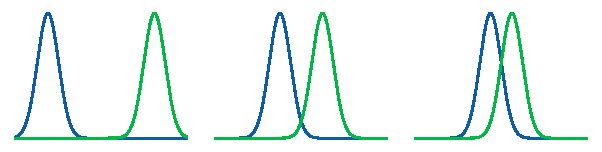
\includegraphics{bilder/plots/theo-vis/gauss-overlap.pdf}
    \caption{Wahrscheinlichkeitsdichte für verschiedene Abstände zwischen zwei gaußverteilten Zuständen \label{fig:gauß-overlap}}
\end{figure}

Viele Algorithmen, die versuchen die Zustände zu bestimmen, haben das Problem, dass sie bei einem Übergang von einem Zustand in den anderen, kurzzeitig zwischen den Zuständen hin und her springen. Dieses \enquote{overshooting} sorgt für eine hohe Anzahl an Zustandswechseln im extrahieren Telegrafenrauschen, die nicht real sind.

\begin{figure}[h]
    \centering
    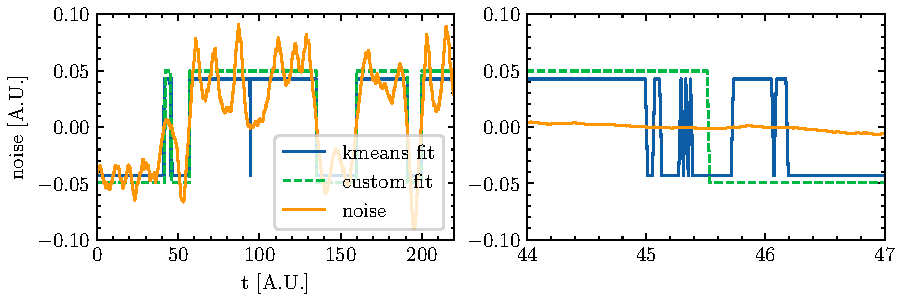
\includegraphics{bilder/plots/theo-vis/telegraph_fit_comp.pdf}
    \caption{Vergleich von Kmeans (mit \(n=2\)) mit einem eigenen Algorithmus. Bei beiden Plots handelt es sich um einen Ausschnitt aus einer größeren Datenreihe. Bei dem kleineren Intervall (rechter Plot) erkennt man gut das Problem, das bei jedem neuen Datenpunkt das Niveau gewechselt wird}\label{fig:fit_comp}
\end{figure}

In \cite{random-telegraph-analysis} wird ein recht komplexer Algorithmus vorgestellt, der in der Lage ist, eine Telegrafenrauschen Kurve in zwei Zustände zu unterteilen, ohne zum overshooting zu neigen. Für die Analyse der Simulationen wird eine modifizierte Version dieses Algorithmus verwendet, die weniger komplex ist, aber für die Analyse der Simulationen ausreicht.

Als erstes wird ein Histogramm der Rauschkurve (\cref{fig:hist_fit}) erstellt (so normiert, das es der Wahrscheinlichkeitsdichte entspricht). \label{sec:algo}
Das erste und das letzte drittel des Histogramms werden dann jeweils mit einer Gaußkurve gefittet, um so die Mittelwerte und die Standardabweichungen der beiden Zustände zu bestimmen.

\begin{figure}[h]
    \centering
    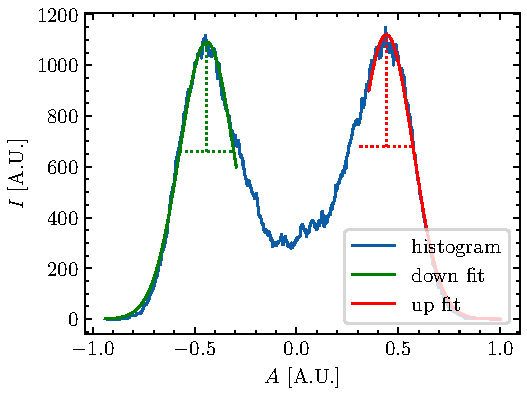
\includegraphics{bilder/plots/theo-vis/hist_fit.pdf}
    \caption{Histogramm des Rauschsignals aus \cref{fig:fit_comp} mit Gaußfits für das obere, und das untere Niveau mit eingezeichnetem Mittelwert und Standardabweichung\todo{auch in Wahrscheinlichkeitsdichteverteilung?}}
    \label{fig:hist_fit}
\end{figure}

Anhand dieser Werte werden dann zwei Schwellwerte bestimmt, die angeben, wann der Zustand gewechselt wird.

Diese Schwellwerte sind definiert als \(x_0 \pm 3\sigma\). Falls die zwei zustände zu weit auseinander liegen, werden sie so lange verschoben, bis sie sich überlappen. 
In dem Fall ist es eigentlich sehr einfach zu entscheiden, in welchem Zustand sich das System gerade befindet, aber der Algorithmus ist auf sich überlappende Zustände ausgelegt.

Es ergeben sich also zwei (sich überlappende) Intervalle, welche jeweils einem Zustand zugeordnet werden.

\begin{figure}[h]
    \centering
    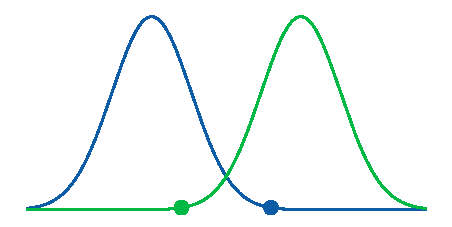
\includegraphics{bilder/plots/theo-vis/bounds.pdf}
    \caption{Zwei sich überlappende gaußverteilte Zustände (wie in \cref{fig:gauss-overlap}) mit den sich überlappenden Intervallgrenzen (bei \(3\sigma\)) eingezeichnet }
\end{figure}


Es wird angenommen, dass sich das System am Anfang (Nullter Datenpunkt) im ersten Zustand befindet.

Dann wird jeder Datenpunkt der Rauschkurve durchgegangen. Nur, wenn der Datenpunkt sich nicht im Intervall, welches dem aktuellen Zustand zugeordnet ist, befindet, wird der Zustand gewechselt. 

Dadurch, dass die Aufenthaltszeit in einem der Zustände deutlich größer ist, als die in der zwischen den Zuständen gewechselt wird, sollte es kein Problem sein, dass sehr Kurze Hin- und Zurückwechsel teilweise vernachlässigt werden. 

\subsection{Fouriertransformation}

Für die Analyse in der Frequenzdomäne wird die diskrete Fouriertransformation
benötigt. Dafür wird die \enquote{fast Fourier transformation} (FFT) verwendet,
welche die Berechnung der Fouriertransformation mit einer Laufzeit von
$\mathcal{O}(n \log n)$ ermöglicht. Die FFT ist in der Bibliothek
\texttt{numpy} \cite{numpy-fft} implementiert.

Die diskrete Fouriertransformation einer Funktion $a_m$ mit $m = 0, \dots, n-1$
ist definiert als:
\begin{align}
    A_k = \sum_{m=0}^{n-1} a_m \exp(-2 \pi i\frac{ k m}{n}) \quad \text{mit}
    \quad k = 0, \dots, n-1
\end{align}

und die inverse Fouriertransformation als:

\begin{align}
    a_m = \frac{1}{n} \sum_{k=0}^{n-1} A_k \exp(2 \pi i\frac{ k m}{n}) \quad
    \text{mit} \quad m = 0, \dots, n-1
\end{align}

\todo{Mittlung der Fouriertransformierten (lieber konstante Anzahl an Segmenten, oder den runs entsprechend) \cref{fig:spd-seg}}


% Korelationsfunktion?

% bibliography (temporary)
% \bibliography{literatur} \todo{comment out before compiling main.tex}

\end{document}